\documentclass[10pt,openright,twoside,french]{book}
\input philippe2013
\input philippe2013_activites
\pagestyle{empty}


\begin{document}

\TitreActivite{ii.3}{Représentation graphique \par de fonctions composées}

Le plan est muni du repère orthonormal \Oij. On définit la fonction $u$ sur l'intervalle $\intervalleff{-2}{4}$ dont on donne la représentation graphique $\calig C$ ci-dessous.

\begin{center}
	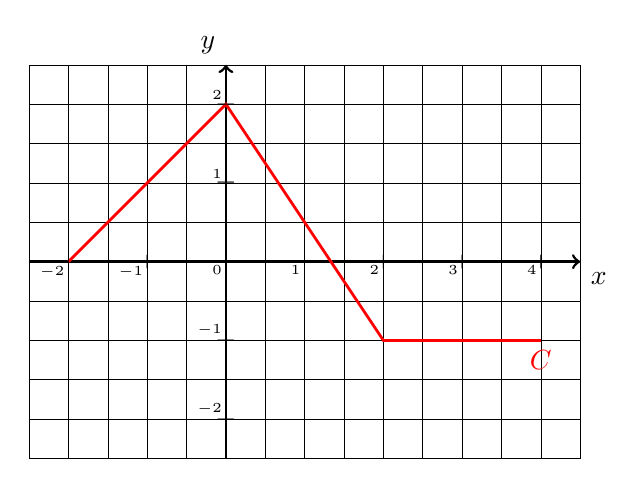
\begin{tikzpicture}
		\draw[line width = 0.2pt] (-2.5,-2.5) grid[xstep=0.5,ystep=0.5] (4.5,2.5);
		\draw[line width = 1pt,->] (-2.5,0)--(4.5,0) node[below right] {$x$};
		\draw[line width = 1pt,->] (0,-2.5)--(0,2.5) node[above left] {$y$};
		\draw[line width=1pt,color=red] (-2,0) -- (0,2) -- (2,-1) -- (4,-1) node[below] {$\calig C$};
		\foreach \x in {-2,-1,...,4} \draw(\x,0) node {\tiny$\vert$} node[below left=-2pt] {\tiny $\x$};
		\foreach \x in {-2,-1} \draw(0,\x) node {$-$} node[above left=-2pt] {\tiny $\x$};
		\foreach \x in {2,1} \draw(0,\x) node {$-$} node[above left=-2pt] {\tiny $\x$};
	\end{tikzpicture}
\end{center}

\section*{Fonction $u + k$}
\begin{enumerate}
	\item Compléter le tableau suivant :
	\begin{center}
		\renewcommand{\arraystretch}{1.5}
		\begin{tabular}{|c|*{7}{>{\centering\arraybackslash}m{1cm}|}}
			\hline
				$x$ & $-2$ & $-1$ & $0$ & $1$ & $2$ & $3$ & $4$ \\
			\hline
				$u(x)$ & & & & & & & \\
			\hline
				$f(x) = u(x) + 1$ & & & & & & & \\
			\hline
				$g(x) = u(x) - 2$ & & & & & & & \\
			\hline
		\end{tabular}
	\end{center}
	\item Sur le repère ci-dessous, construire \textbf{en rouge} la courbe $\calig C_1$ représentative de $f$ et \textbf{en vert} la courbe $\calig C_2$ représentative de $g$.
	\item Indiquer comment obtenir $\calig C_1$ et $\calig C_2$ en fonction de $\calig C$.
\end{enumerate}\medskip

\begin{center}
	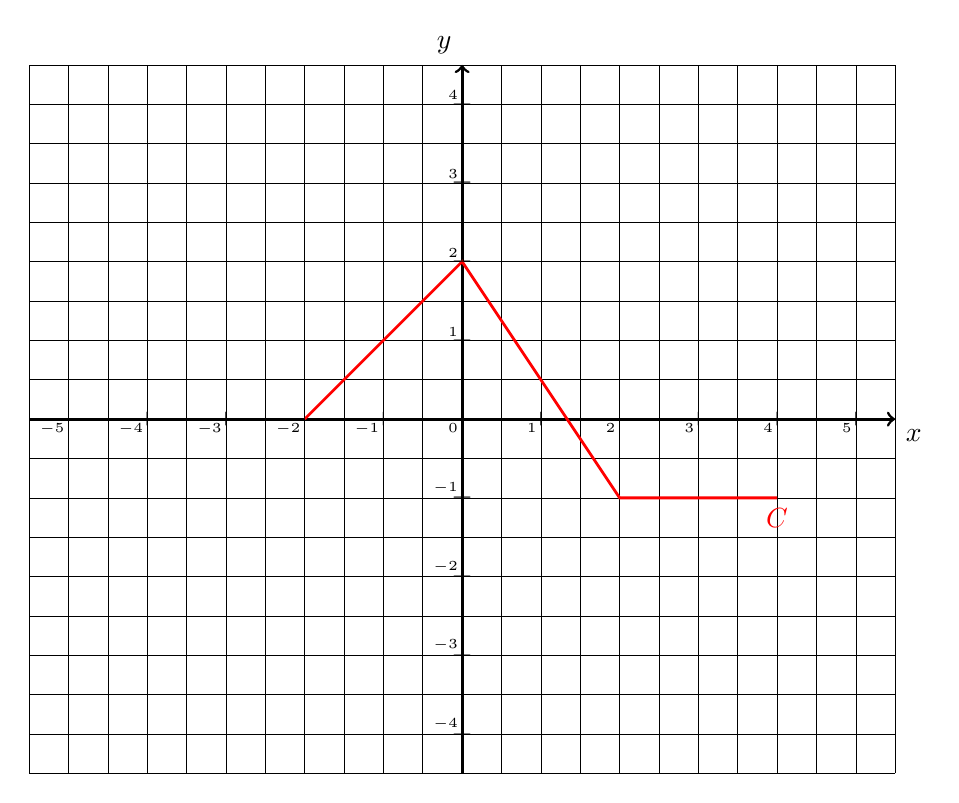
\begin{tikzpicture}
		\draw[line width = 0.2pt] (-5.5,-4.5) grid[xstep=0.5,ystep=0.5] (5.5,4.5);
		\draw[line width = 1pt,->] (-5.5,0)--(5.5,0) node[below right] {$x$};
		\draw[line width = 1pt,->] (0,-4.5)--(0,4.5) node[above left] {$y$};
		\draw[line width=1pt,color=red] (-2,0) -- (0,2) -- (2,-1) -- (4,-1) node[below] {$\calig C$};
		\foreach \x in {-5,-4,...,5} \draw(\x,0) node {\tiny$\vert$} node[below left=-2pt] {\tiny $\x$};
		\foreach \x in {-4,-3,...,-1} \draw(0,\x) node {$-$} node[above left=-2pt] {\tiny $\x$};
		\foreach \x in {1,2,...,4} \draw(0,\x) node {$-$} node[above left=-2pt] {\tiny $\x$};
	\end{tikzpicture}
\end{center}

\section*{Fonction $t \mapsto u(t + \lambda)$}

\begin{enumerate}
	\item Sur le repère ci-dessous, construire en vert la courbe $\calig C_3$ obtenue par une translation \textbf{horizontale} de tous les points de $\calig C$ d'une unité \textbf{vers la gauche}.
	\item On appelle $h$ la fonction dont la représentation graphique est $\calig C_3$.
	\begin{enumerate}
		\item Sur quel intervalle $I_1$ la fonction $h$ est-elle définie ?
		\item Pour les valeurs entières de $I_1$, a-t-on $h(t) = u(t + 1)$ ou $h(t) = u(t - 1)$ ?
	\end{enumerate}
	\item Toujours sur le repère ci-dessous, construire en bleu la courbe $\calig C_4$ obtenue par une translation \textbf{horizontale} de tous les points de $\calig C$ de deux unités \textbf{vers la droite}.
	\item On appelle $\ell$ la fonction dont la représentation graphique est $\calig C_4$.
	\begin{enumerate}
		\item Sur quel intervalle $I_2$ la fonction $\ell$ est-elle définie ?
		\item Pour les valeurs entières de $I_2$, a-t-on $\ell(t) = u(t + 2)$ ou $\ell(t) = u(t - 2)$ ?
	\end{enumerate}
\end{enumerate}

\begin{center}
	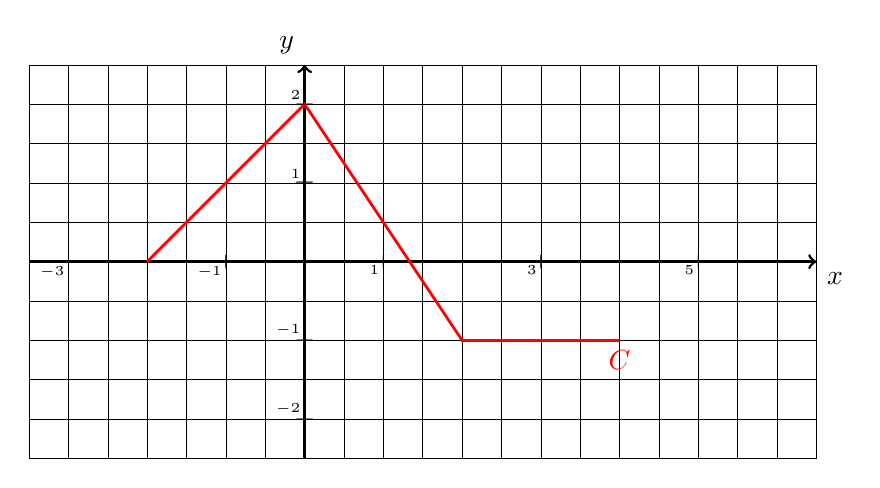
\begin{tikzpicture}
		\draw[line width = 0.2pt] (-3.5,-2.5) grid[xstep=0.5,ystep=0.5] (6.5,2.5);
		\draw[line width = 1pt,->] (-3.5,0)--(6.5,0) node[below right] {$x$};
		\draw[line width = 1pt,->] (0,-2.5)--(0,2.5) node[above left] {$y$};
		\draw[line width=1pt,color=red] (-2,0) -- (0,2) -- (2,-1) -- (4,-1) node[below] {$\calig C$};
		\foreach \x in {-3,-1,...,6} \draw(\x,0) node {\tiny$\vert$} node[below left=-2pt] {\tiny $\x$};
		\foreach \x in {-2,-1} \draw(0,\x) node {$-$} node[above left=-2pt] {\tiny $\x$};
		\foreach \x in {2,1} \draw(0,\x) node {$-$} node[above left=-2pt] {\tiny $\x$};
	\end{tikzpicture}
\end{center}

\section*{Fonction $\abs u$}
\begin{enumerate}
	\item Compléter le tableau suivant :
	\begin{center}
		\renewcommand{\arraystretch}{1.5}
		\begin{tabular}{|c|*{7}{>{\centering\arraybackslash}m{1cm}|}}
			\hline
				$x$ & $-2$ & $-1$ & $0$ & $1$ & $2$ & $3$ & $4$ \\
			\hline
				$u(x)$ & & & & & & & \\
			\hline
				$m(x) = \abs{u(x)}$ & & & & & & & \\
			\hline
		\end{tabular}
	\end{center}
	\item Sur le repère ci-dessous, construire \textbf{en rouge} la courbe $\calig C_5$ représentative de $m$.
	\item Quel est le signe de $m$ ?
\end{enumerate}\medskip

\begin{center}
	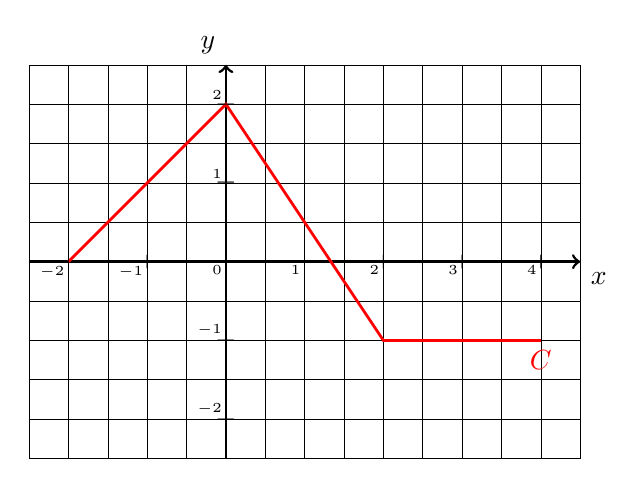
\begin{tikzpicture}
		\draw[line width = 0.2pt] (-2.5,-2.5) grid[xstep=0.5,ystep=0.5] (4.5,2.5);
		\draw[line width = 1pt,->] (-2.5,0)--(4.5,0) node[below right] {$x$};
		\draw[line width = 1pt,->] (0,-2.5)--(0,2.5) node[above left] {$y$};
		\draw[line width=1pt,color=red] (-2,0) -- (0,2) -- (2,-1) -- (4,-1) node[below] {$\calig C$};
		\foreach \x in {-2,-1,...,4} \draw(\x,0) node {\tiny$\vert$} node[below left=-2pt] {\tiny $\x$};
		\foreach \x in {-2,-1} \draw(0,\x) node {$-$} node[above left=-2pt] {\tiny $\x$};
		\foreach \x in {2,1} \draw(0,\x) node {$-$} node[above left=-2pt] {\tiny $\x$};
	\end{tikzpicture}
\end{center}

\end{document} 